% Options for packages loaded elsewhere
\PassOptionsToPackage{unicode}{hyperref}
\PassOptionsToPackage{hyphens}{url}
\PassOptionsToPackage{dvipsnames,svgnames,x11names}{xcolor}
%
\documentclass[
  11pt,
  dvipsnames,enabledeprecatedfontcommands]{scrartcl}
\usepackage{amsmath,amssymb}
\usepackage{lmodern}
\usepackage{iftex}
\ifPDFTeX
  \usepackage[T1]{fontenc}
  \usepackage[utf8]{inputenc}
  \usepackage{textcomp} % provide euro and other symbols
\else % if luatex or xetex
  \usepackage{unicode-math}
  \defaultfontfeatures{Scale=MatchLowercase}
  \defaultfontfeatures[\rmfamily]{Ligatures=TeX,Scale=1}
\fi
% Use upquote if available, for straight quotes in verbatim environments
\IfFileExists{upquote.sty}{\usepackage{upquote}}{}
\IfFileExists{microtype.sty}{% use microtype if available
  \usepackage[]{microtype}
  \UseMicrotypeSet[protrusion]{basicmath} % disable protrusion for tt fonts
}{}
\usepackage{xcolor}
\IfFileExists{xurl.sty}{\usepackage{xurl}}{} % add URL line breaks if available
\IfFileExists{bookmark.sty}{\usepackage{bookmark}}{\usepackage{hyperref}}
\hypersetup{
  pdftitle={Beyond Reverse Bayesianism:},
  pdfauthor={Marcello Di Bello and Rafal Urbaniak},
  colorlinks=true,
  linkcolor={Maroon},
  filecolor={Maroon},
  citecolor={Blue},
  urlcolor={blue},
  pdfcreator={LaTeX via pandoc}}
\urlstyle{same} % disable monospaced font for URLs
\usepackage{graphicx}
\makeatletter
\def\maxwidth{\ifdim\Gin@nat@width>\linewidth\linewidth\else\Gin@nat@width\fi}
\def\maxheight{\ifdim\Gin@nat@height>\textheight\textheight\else\Gin@nat@height\fi}
\makeatother
% Scale images if necessary, so that they will not overflow the page
% margins by default, and it is still possible to overwrite the defaults
% using explicit options in \includegraphics[width, height, ...]{}
\setkeys{Gin}{width=\maxwidth,height=\maxheight,keepaspectratio}
% Set default figure placement to htbp
\makeatletter
\def\fps@figure{htbp}
\makeatother
\setlength{\emergencystretch}{3em} % prevent overfull lines
\providecommand{\tightlist}{%
  \setlength{\itemsep}{0pt}\setlength{\parskip}{0pt}}
\setcounter{secnumdepth}{5}
%\documentclass{article}

% %packages
\usepackage{booktabs}
%\usepackage[left]{showlabels}
\usepackage{multirow}
\usepackage{subcaption}
\usepackage{wrapfig}
\usepackage{graphicx}
\usepackage{longtable}
\usepackage{ragged2e}
\usepackage{etex}
%\usepackage{yfonts}
\usepackage{marvosym}
\usepackage[notextcomp]{kpfonts}
\usepackage{nicefrac}
\newcommand*{\QED}{\hfill \footnotesize {\sc Q.e.d.}}
\usepackage{floatrow}
\usepackage{multicol}

\usepackage[textsize=footnotesize]{todonotes}
\newcommand{\ali}[1]{\todo[color=gray!40]{\textbf{Alicja:} #1}}
\newcommand{\mar}[1]{\todo[color=blue!40]{#1}}
\newcommand{\raf}[1]{\todo[color=olive!40]{#1}}

%\linespread{1.5}
\newcommand{\indep}{\!\perp \!\!\! \perp\!}


\setlength{\parindent}{10pt}
\setlength{\parskip}{1pt}


%language
%\usepackage{times}
\usepackage{mathptmx}
\usepackage[scaled=0.86]{helvet}
\usepackage{t1enc}
%\usepackage[utf8x]{inputenc}
%\usepackage[polish]{babel}
%\usepackage{polski}




%AMS
\usepackage{amsfonts}
\usepackage{amssymb}
\usepackage{amsthm}
\usepackage{amsmath}
\usepackage{mathtools}

\usepackage{geometry}
 \geometry{a4paper,left=35mm,top=20mm,}


%environments
\newtheorem{fact}{Fact}


% allow page breaks in equations
\allowdisplaybreaks


%abbreviations
\newcommand{\ra}{\rangle}
\newcommand{\la}{\langle}
\newcommand{\n}{\neg}
\newcommand{\et}{\wedge}
\newcommand{\jt}{\rightarrow}
\newcommand{\ko}[1]{\forall  #1\,}
\newcommand{\ro}{\leftrightarrow}
\newcommand{\exi}[1]{\exists\, {_{#1}}}
\newcommand{\pr}[1]{\ensuremath{\mathsf{P}(#1)}}
\newcommand{\ppr}[2]{\ensuremath{\mathsf{P}^{#1}(#2)}}
\newcommand{\cost}{\mathsf{cost}}
\newcommand{\benefit}{\mathsf{benefit}}
\newcommand{\ut}{\mathsf{ut}}

\newcommand{\odds}{\mathsf{Odds}}
\newcommand{\ind}{\mathsf{Ind}}
\newcommand{\nf}[2]{\nicefrac{#1\,}{#2}}
\newcommand{\R}[1]{\texttt{#1}}
\newcommand{\prr}[1]{\mbox{$\mathtt{P}_{prior}(#1)$}}
\newcommand{\prp}[1]{\mbox{$\mathtt{P}_{posterior}(#1)$}}



\newtheorem{q}{\color{blue}Question}
\newtheorem{lemma}{Lemma}
\newtheorem{theorem}{Theorem}
\newtheorem{corollary}{Corollary}[fact]


%technical intermezzo
%---------------------

\newcommand{\intermezzoa}{
	\begin{minipage}[c]{13cm}
	\begin{center}\rule{10cm}{0.4pt}



	\tiny{\sc Optional Content Starts}
	
	\vspace{-1mm}
	
	\rule{10cm}{0.4pt}\end{center}
	\end{minipage}\nopagebreak 
	}


\newcommand{\intermezzob}{\nopagebreak 
	\begin{minipage}[c]{13cm}
	\begin{center}\rule{10cm}{0.4pt}

	\tiny{\sc Optional Content Ends}
	
	\vspace{-1mm}
	
	\rule{10cm}{0.4pt}\end{center}
	\end{minipage}
	}
	
	
%--------------------






















\newtheorem*{reply*}{Reply}
\usepackage{enumitem}
\newcommand{\question}[1]{\begin{enumerate}[resume,leftmargin=0cm,labelsep=0cm,align=left]
\item #1
\end{enumerate}}

\usepackage{float}

% \setbeamertemplate{blocks}[rounded][shadow=true]
% \setbeamertemplate{itemize items}[ball]
% \AtBeginPart{}
% \AtBeginSection{}
% \AtBeginSubsection{}
% \AtBeginSubsubsection{}
% \setlength{\emergencystretch}{0em}
% \setlength{\parskip}{0pt}






\usepackage[authoryear]{natbib}

%\bibliographystyle{apalike}



\usepackage{tikz}
\usetikzlibrary{positioning,shapes,arrows}

\ifLuaTeX
  \usepackage{selnolig}  % disable illegal ligatures
\fi

\title{Beyond Reverse Bayesianism:}
\usepackage{etoolbox}
\makeatletter
\providecommand{\subtitle}[1]{% add subtitle to \maketitle
  \apptocmd{\@title}{\par {\large #1 \par}}{}{}
}
\makeatother
\subtitle{Awareness Growth and Bayesian Networks}
\author{Marcello Di Bello and Rafal Urbaniak}
\date{June 13, 2022}

\begin{document}
\maketitle

\hypertarget{introduction}{%
\section{Introduction}\label{introduction}}

Learning is modeled in the Bayesian framework by the rule of
conditionalization. This rule posits that the agent's new degree of
belief in a proposition \(H\) after a learning experience \(E\) should
be the same as the agent's old degree of belief in \(H\) conditional on
\(E\). That is, \[\ppr{E}{H}=\pr{H \vert E},\] where \(\pr{}\)
represents the agent's old degree of belief (before the learning
experience \(E\)) and \(\ppr{E}{}\) represents the agent's new degree of
belief (after the learning experience \(E\)).

Both \(E\) and \(H\) belong to the agent's algebra of propositions. This
algebra models the agent's awareness state, the propositions taken to be
live possibilities. Conditionalization never modifies the algebra and
thus makes it impossible for an agent to learn something they have never
thought about. This forces a great deal of rigidity on the learning
process. Even before learning about \(E\), the agent must already have
assigned a degree of belief to any proposition conditional on \(E\).
This picture commits the agent to the specification of their `total
possible future experience' (Howson 1976, The Development of Logical
Probability), as though learning was confined to an `initial prison'
(Lakatos, 1968, Changes in the Problem of Inductive Logic).

But, arguably, the learning process is more complex than what
conditionalization allows. Not only do we learn that some propositions
that we were entertaining are true or false, but we may also learn new
propositions that we did not entertain before. Or we may entertain new
propositions---without necessarily learning that they are true or
false---and this change in awareness may in turn change what we already
believe. How should this more complex learning process be modeled by
Bayesianism? Call this the problem of awareness growth.

Critics of Bayesianism and sympathizers alike have been discussing the
problem of awareness growth under different names for quite some time,
at least since the eighties. This problem arises in a number of
different contexts, for example, new scientific theories (Glymour, 1980,
Why I am not a Bayesian; Chihara 1987, Some Problems for Bayesian
Confirmation Theory; Earmann 1992, Bayes of Bust?), language changes and
paradigm shifts (Williamson 2003, Bayesianism and Language Change), and
theories of induction (Zabell, Predicting the Unpredictable).

Now, of course, the algebra of propositions could in principle be so
rich to contain anything that could possibly be conceived, expressed,
thought of. Such an algebra would not need to change at any point in the
future. God-like agents could be associated with such rich algebra of
propositions, but this is hardly a plausible model of ordinary agents
with bounded resources such as ourselves. To be sure, the algebra of
propositions need not be so narrowly construed that it only contains
propositions that are presently under consideration. The algebra may
also contain propositions about which, even though they are not the
object to present consideration, the agent has already formed, perhaps
simplicity, a certain disposition to believe. If, however, we have
actual applications of probabilistic tools in mind, this is not a
promising strategy. We are not God-like agents, probabilistic models are
small-world models always restricted to a pre-specified set of
variables, and some guidance as to how these should be revised when our
awareness changes without the unrealistic assumption of us already
having had the right algebra and probabilities to start with is
desirable.

A proposal that has attracted considerable scholarly attention in recent
years is Reverse Bayesianism (Karni and Viero, 2015, Probabilistic
Sophistication and Reverse Bayesianism; Wenmackers and Romeijn 2016, New
Theory About Old Evidence; Bradely 2017, Decision Theory with A Human
Face) . The idea is to model awareness growth as a change in the algebra
while ensuring that the proportions of probabilities of the propositions
shared between the old and new algebra remain the same in the sense to
be specified.

Let \(\mathcal{F}\) be the initial algebra of propositions and let
\(\mathcal{F}^+\) the algebra after the agent's awareness state has
grown. Both algebras contain the contradictory and tautologous
propositions \(\perp\) and \(\top\), and they are closed under
connectives such as disjunction \(\vee\), conjunction \(\wedge\) and
negation \(\neg\). Denote by \(X\) and \(X^+\) the subsets of these
algebras that contain only basic propositions, namely those without
connectives. \textbf{Reverse Bayesianism} posits that the ratio of
probabilities for any basic propositions \(A\) and \(B\) in both \(X\)
and \(X^+\)---the basic propositions shared by the old and new
algebra---remain constant through the process of awareness growth:
\[\frac{\pr{A}}{\pr{B}} = \frac{\ppr{+}{A}}{\ppr{+}{B}},\] where
\(\pr{}\) represents the agent's degree of belief before awareness
growth and \(\ppr{+}{}\) represents the agent's degree of belief after
awareness growth.

Reverse Bayesianism is an elegant theory that manages to cope with a
seemingly intractable problem. As the awareness state of an an agent
grows, the agent would prefer not to throw away completely the epistemic
work they have done so far. The agent may desire to retain as much of
their old degrees of beliefs as possible. Reverse Bayesianism provides a
simple recipe to do that. It also coheres with the conservative spirit
of conditionalization which preserves the old probability distribution
conditional on what is learned.

Unfortunately, Reverse Bayesianism is not without complications. Steele
and Stefánsson (2021, Belief Revision for Growing Awareness) argue that
Reverse Bayesianism, when suitably formulated, can work in a limited
class of cases, what they call \textit{awareness expansion}, but cannot
work for \textit{awareness refinement} (more on this distinction later).
Their argument rests on a number of ingenious counterexamples.

We share Steele and Stefánsson's skepticism toward Reverse Bayesianism,
but also believe their counterexamples have limited applicability. We
strengthen their argument by providing a simpler counterexample that is
less prone to objections (\S ~\ref{sec:counterexamples}) . At the same
time, we conjecture that the problem of awareness growth cannot be
tackled in an algorithmic manner because subject-matter assumptions,
both probabilistic and structural, need to be made explicit. Thanks to
its ability to model probabilistic dependencies, we think that the
theory of Bayesian networks can help to theorize about awareness growth
in the Bayesian framework. We offer two illustrations of this claim.
First, we provide an example of awareness growth refinement that it is
structurally different from other cases of refinement
(\S ~\ref{sec:downstream}). Second, we model two scenarios from Anna
Mathani, both intended to challenge Reverse Bayesianism
(\S ~\ref{sec:mathani}). As we will see, Bayesian networks allow us to
see more clearly which probability assignments should be retained during
awareness growth and which ones should be modified. The choice is guided
by the underlying structure of the scenarios, requires material
knowledge and does not fall out from purely formal constraints.

\hypertarget{counterexamples}{%
\section{Counterexamples}\label{counterexamples}}

\label{sec:counterexamples} \label{sec:better}

We begin by rehearsing two of the ingenious counterexamples to Reverse
Bayesianism by Steele and Stefánsson. One example targets awareness
expansion and the other awareness refinement. The difference between
expansion and refinement is intuitively plausible, but it can be tricky
to pin down formally. A rough characterization will suffice here.
Suppose, as is customary, propositions are interpreted as sets of
possible worlds, where the set of all possible worlds is the possibility
space. An algebra of propositions thus interpreted induces a partition
of the possibility space. Refinement occurs when the new proposition
added to the algebra induces a more fine-grained partition of the
possibility space. Expansion, instead, occurs when the new proposition
shows that the existing partition was not exhaustive.

The first counterexample by Steele and Stefánsson targets cases of
awareness expansion:

\begin{quote}
\textsc{Friends}: Suppose you happen to see your partner enter your best
friend's house on an evening when your partner had told you she would
have to work late. At that point, you become convinced that your partner
and best friend are having an affair, as opposed to their being warm
friends or mere acquaintances. You discuss your suspicion with another
friend of yours, who points out that perhaps they were meeting to plan a
surprise party to celebrate your upcoming birthday---a possibility that
you had not even entertained. Becoming aware of this possible
explanation for your partner's behaviour makes you doubt that she is
having an affair with your friend, relative, for instance, to their
being warm friends. (Steele and Stefánsson, 2021, Section 5, Example 2)
\end{quote}

\noindent Initially, the algebra only contains the hypotheses `my
partner and my best friend met to have an affair' (\textit{Affair}) and
`my partner and my best friend met as friends or acquaintances'
(\textit{Friends/acquaintances}). The other proposition in the algebra
is the evidence, that is, the fact that your partner and your best
friend met one night without telling you (\textit{Secretive}). Given
this evidence, \textit{Affair} is more probable than
\textit{Friends/acquaintances}:
\[\pr{\textit{Affair} \vert  \textit{Secretive} }> \pr{\textit{Friends/acquaintances} \vert \textit{Secretive}} \tag{>}.\]
When the algebra changes, a new hypothesis is added which you had not
considered before: your partner and your best friends met to plan a
surprise party for your upcoming birthday (\textit{Surprise}). Given the
same evidence, \textit{Friends/acquaintances} is now more likely than
\textit{Affair}:
\[\ppr{+}{\textit{Affair} \vert  \textit{Secretive} } < \ppr{+}{\textit{Friends/acquaintances} \vert \textit{Secretive}}. \tag{<}\]
This holds assuming that hypothesis \textit{Surprise} is more likely
than the hypothesis \textit{Affair}:
\[\ppr{+}{ \textit{Surprise} \vert \textit{Secretive}}> \ppr{+}{ \textit{Affair} \vert \textit{Secretive}},\]
and, in addition, that \textit{Surprise} implies
\textit{Friends/acquaintances}. After all, in order to prepare a
surprise party, your partner and best friend have to be at least
acquaintances.

The conjunction of (\(>\)) and (\(<\)) violates Reverse Bayesianism.
But, as Steele and Stefánsson admits, Reverse Bayesianism can still be
made to work with a slightly different---though quite similar in
spirit---condition, called \textbf{Awareness Rigidity}:
\[\ppr{+}{A \vert T^*}=\pr{A},\] where \(T^*\) corresponds to a
proposition that picks out, from the vantage point of the new awareness
state, the entire possibility space before the episode of awareness
growth. In our running example, the proposition
\(\neg\textit{Surprise}\) picks out the entire possibility space in just
this way. And conditional on \(\neg\textit{Surprise}\), the probability
of \textit{Affair} does not change. Thus,
\[\ppr{+}{\textit{Affair} \vert  \textit{Secretive} \& \neg\textit{Surprise} } > \ppr{+}{\textit{Friends/acquaintances} \vert \textit{Secretive} \& \neg\textit{Surprise}}. \]
Awareness Rigidity is satisfied. Reverse Bayesianism---the spirit of it,
not the letter---stands.

This is not the end of the story, however. Steele and Stefánsson offer
another counterexample that also works against Awareness Rigidity, this
time targeting a case of refinement:

\begin{quote}
\textsc{Movies}: Suppose you are deciding whether to see a movie at your
local cinema. You know that the movie's predominant language and genre
will affect your viewing experience. The possible languages you consider
are French and German and the genres you consider are thriller and
comedy. But then you realise that, due to your poor French and German
skills, your enjoyment of the movie will also depend on the level of
difficulty of the language. Since it occurs to you that the owner of the
cinema is quite simple-minded, you are, after this realisation, much
more confident that the movie will have low-level language than
high-level language. Moreover, since you associate low-level language
with thrillers, this makes you more confident than you were before that
the movie on offer is a thriller as opposed to a comedy. (Steele and
Stefánsson, 2021, Section 5, Example 3)
\end{quote}

\noindent Initially, you did not consider language difficulty. So you
assigned the same probability to the hypotheses \textit{Thriller} and
\textit{Comedy}. But learning that the owner is simple-minded made you
think that the level of linguistic difficulty must be low and the movie
most likely a thriller rather than a comedy (perhaps because thrillers
are simpler---linguistically---than comedies). So, against Reverse
Bayesianism, \textsc{Movies} violates the condition
\(\frac{\pr{\textit{Thriller}}}{\pr{\textit{Comedy}}}=\frac{\ppr{+}{\textit{Thriller}}}{\ppr{+}{\textit{Comedy}}}\).

The counterexample also works against Awareness Rigidity. It is not true
that
\(\pr{\textit{Thriller}}=\ppr{+}{\textit{Thriller} \vert \textit{Thriller}\vee \textit{Comedy}}\).
Note that this counterexample is a case of refinement. First, you
categorize movies by just language and genre, and then you add a further
category, level of difficulty. So the proposition which picks out the
entire possibility space should be the same before and after awareness
growth, for example, \(\textit{Thriller}\vee \textit{Comedy}\). In cases
of awareness growth by refinement, then, Awareness Rigidity mandates
that all probability assignments stay the same. But \textsc{Movies} does
not satisfy this requirement.

This is all well and good, but how strong of a counterexample is this?
Steele and Stefánsson consider an objection:

\begin{quote}It might be argued that our examples are not illustrative of \dots a simple growth in awareness; rather, our examples illustrate and should be expressed 
  formally as complex learning experiences, where first there is a growth in awareness, and then 
  there is a further learning event ... In this way, one could argue that the awareness-growth 
  aspect of the learning event always satisfies Reverse Bayesianism.
\end{quote}

\noindent  Admittedly, \textsc{Movies} can be split into two episodes.
In the first, you entertain a new variable besides language and genre,
namely the language difficulty of the movie. In the second episode, you
learn something you did not consider before, namely that the owner is
simple-minded. Could Reserve Bayesianism still work for the first
episode, but not the second? Steele and Stefánsson do not address this
question explicitly, but insist that no matter the answer both episodes
are instances of awareness growth. We agree with them on this point.
Awareness growth is both \textit{entertaining} a new proposition not in
the initial awareness state of the agent and \textit{learning} a new
proposition. Nonetheless, we should still wonder. Is the second episode
(learning something new) necessary for the counterexample to work
together with the first episode (mere refinement without learning)?

Suppose the counterexample did work only in tandem with an episode of
learning something new. If that were so, defenders of Reverse
Bayesianism or Awareness Rigidity could still claim that their theory
applies to a large class of cases. It applies to cases of awareness
refinement without learning and also to cases of awareness expansion.
For recall that the first putative counterexample featuring awareness
expansion---\textsc{Friends}---did not challenge Reverse Bayesianism
insofar as the latter is formulated in terms of its close cousin,
Awareness Rigidity. So the force of Steele and Stefánsson's
counterexamples would be rather limited.

Or perhaps there is a more straightforward counterexample that only
depicts mere refinement without an episode of learning and that still
challenges Reverse Bayesianism and Awareness Rigidity. This is indeed
the case, as this scenario illustrates:

\begin{quote}
\textsc{Lighting:} You have evidence that favors a certain hypothesis,
say a witness saw the defendant around the crime scene. You give some
weight to this evidence. In your assessment, that the defendant was seen
around the crime scene raises the probability that the defendant was
actually there. But now you wonder, what if it was dark when the witness
saw the defendant? You become a bit more careful and settle on this: if
the lighting conditions were good, you should still trust the evidence,
but if they were bad, you should not. Unfortunately, you cannot learn
about the actual lighting conditions, but the mere realization that it
\textit{could} have been dark makes you lower the probability that the
defendant was actually there, based on the same eveidence.
\end{quote}

\noindent This scenario is simpler because it consists of mere
refinement. You wonder about the lighting conditions but you do not
learn what they were.\footnote{Strictly speaking, you are learning that
  it is \emph{possible} that the lighting conditions were bad. However,
  you do not condition on the proposition `the lighting conditions were
  bad' or `the lighting conditions were good' as if you learned it with
  certainty, and thus you do not learn about the lighting conditions in
  the sense in which learning is understood in this paper.} Still, mere
refinement in this scenario challenges Reverse Bayesianism and Awareness
Rigidity. That this should be so is not easy to see. Fortunately, the
theory of Bayesian networks helps to see why.

A Bayesian network is a formal model that consists of a graph
accompanied by a probability distribution. The nodes in the graph
represent random variables that can take different values. We will use
`nodes' and `variables' interchangeably. The nodes are connected by
arrows, but no loops are allowed, hence the name direct acyclic graph
(DAG). Bayesian networks are relied upon in many fields, but have been
little used to model awareness growth. We think instead they are a good
framework for this purpose. Awareness growth can be modeled as a change
in the graphical network---nodes and arrows are added or erased---as
well as a change in the probability distribution from the old to the new
network.

To model \textsc{Lighting} with Bayesian networks, we start with this
graph, which is the usual hypothesis-evidence idiom:

\begin{center}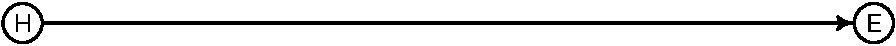
\includegraphics[width=0.5\linewidth,height=0.3\textheight]{ReplyToSteeleStefansson2_files/figure-latex/heDAG-1} \end{center}

where \(H\) is the hypothesis node and \(E\) the evidence node. If an
arrow goes from \(H\) to \(E\), the probability distribution associated
with the Bayesian network should be defined by conditional probabilities
of the form \(\pr{E=e \vert H=h}\), where uppercase letters represent
the variables (nodes) and lower case letters represent the values of
these variables.\footnote{A major point of contention in the
  interpretation of Bayesian networks is is the meaning of the directed
  arrows. They could be interpreted causally---as though the direction
  of causality proceeds from the events described by the hypothesis to
  event described by the evidence---but they need not be. REFERENCES?}
Since you trust the evidence, you think that it is more likely under the
hypothesis that the defendant was present at the crime scene than under
the alternative hypothesis:
\[\pr{\textit{E=seen} \vert \textit{H=present}} > \pr{\textit{E=seen} \vert \textit{H=absent}}\]
The inequality is a qualitative ordering of how plausible the evidence
is in light of competing hypotheses. No matter the numbers, by the
probability calculus, it follows that the evidence raises the
probability of the hypothesis \textit{H=present}.

Now, as you wonder about the lighting conditions, the graph should be
amended:

\begin{center}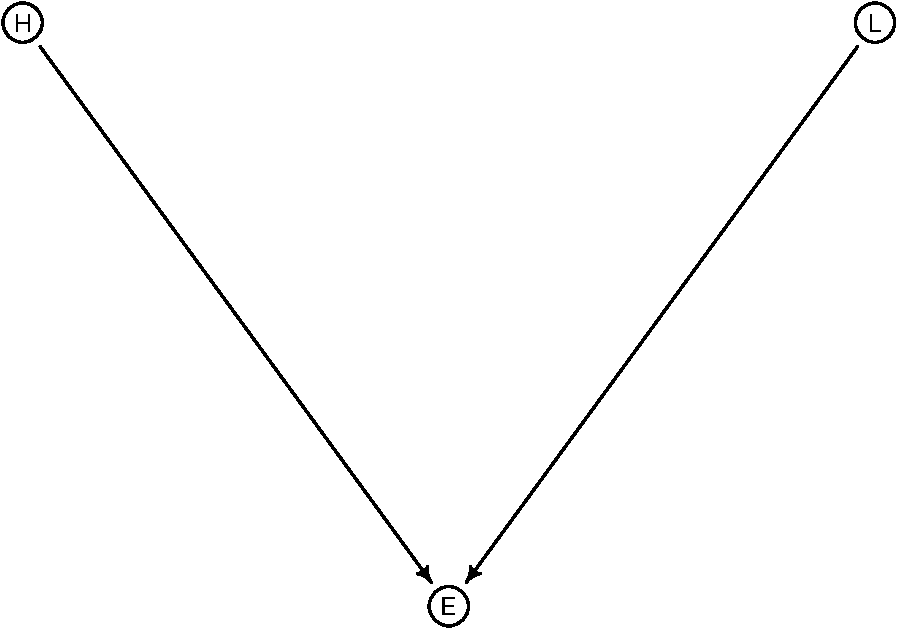
\includegraphics[width=0.5\linewidth,height=0.3\textheight]{ReplyToSteeleStefansson2_files/figure-latex/lighting2DAG-1} \end{center}

\noindent where the node \(L\) can have two values, \textit{L=good} and
\textit{L=bad}. A plausible way to update your assessment of the
evidence is as follows:
\[\ppr{+}{\textit{E=seen} \vert \textit{H=present} \wedge \textit{L=good}} > \ppr{+}{\textit{E=seen} \vert \textit{H=absent} \wedge \textit{L=good}}\]
\[\ppr{+}{\textit{E=seen} \vert \textit{H=present} \wedge \textit{bad}} = \ppr{+}{\textit{E=seen} \vert \textit{H=absent} \wedge \textit{L=bad}}\]

\noindent Note the change in the probability function from \(\pr{}\) to
\(\ppr{+}{}\). Here is what you are thinking: if the lighting conditions
were good, you should still trust the evidence like you did before. But
if the lighting conditions were bad, you should regard the evidence as
no better than chance.

Should you now assess the evidence at your disposal---that the witness
saw the defendant at the crime scene---any differently than you did
before? The evidence would have the same value if the likelihood ratios
associated with it relative to the competing hypotheses were the same
before and after awareness growth:
\[\frac{\pr{E=e \vert H=h}}{\pr{E=e \vert H=h'}}= \frac{\ppr{+}{E=e \vert H=h}}{\ppr{+}{E=e \vert H=h'}} \tag{C}.\]
In our example, many plausible possible probability assignments violate
this equality. But it would be quite a coincidence if (C) were true. If
before awareness growth you thought the evidence favored the hypothesis
\textit{H=present} moderately strongly, after the growth in awareness,
the evidence is likely to appear less strong.\footnote{By the law of
  total probability, the right hand side of the equality should be
  expanded, as follows:
  \[\frac{\ppr{+}{E=e \vert H=h}}{\ppr{+}{E=e \vert H=h'}}=\frac{\ppr{+}{\textit{E=seen} \wedge \textit{L=good} \vert \textit{H=present}}+\ppr{+}{\textit{E=seen} \wedge \textit{L=bad} \vert \textit{H=present}}}{\ppr{+}{\textit{E=seen} \wedge \textit{L=good} \vert \textit{H=absent}}+\ppr{+}{\textit{E=seen} \wedge \textit{L=bad} \vert \textit{H=absent}}}.\]
  For concreteness, let's use some numbers:
  \[\pr{\textit{E=seen} \vert \textit{H=present}}=\ppr{+}{\textit{E=seen} \vert \textit{H=present} \wedge \textit{L=good}}=.8\]
  \[\pr{\textit{E=seen} \vert \textit{H=absent}}=\ppr{+}{\textit{E=seen} \vert \textit{H=absent} \wedge \textit{L=good}}=.4\]
  \[\ppr{+}{\textit{E=seen} \vert \textit{H=present} \wedge \textit{L=bad}} = \ppr{+}{\textit{E=seen} \vert \textit{H=absent} \wedge \textit{L=bad}}=.5.\]
  So the ratio
  \(\frac{\pr{\textit{E=seen} \vert \textit{H=present}}}{\pr{\textit{E=seen} \vert \textit{H=absent}}}\)
  equals \(2\). After the growth in awareness, the ratio
  \(\frac{\ppr{+}{\textit{E=seen} \vert \textit{H=present}}}{\ppr{+}{\textit{E=seen} \vert \textit{H=absent}}}\)
  will drop to \(\frac{.65}{.45}\approx 1.44\). The calculations here
  rely on the dependency structure encoded in the Bayesian network (see
  starred step below). \begin{align*}
  \ppr{+}{\textit{E=seen} \vert \textit{H=present}} &= \ppr{+}{\textit{E=seen} \wedge \textit{L=good} \vert \textit{H=present}}+\ppr{+}{\textit{E=seen} \wedge \textit{L=bad} \vert \textit{H=present}}\\
  &= \ppr{+}{\textit{E=seen} \vert \textit{H=present} \wedge \textit{L=good}}  \times \ppr{+}{\textit{L=good} \vert  \textit{H=present} }\\ & +\ppr{+}{\textit{E=seen}  \vert \textit{H=present} \wedge \textit{L=bad}} \times \ppr{+}{\textit{L=bad} \vert  \textit{H=present}}\\
  &=^* \ppr{+}{\textit{E=seen} \vert \textit{H=present} \wedge \textit{L=good}}  \times \ppr{+}{\textit{L=good}}\\ & +\ppr{+}{\textit{E=seen}  \vert \textit{H=present} \wedge \textit{L=bad}} \times \ppr{+}{\textit{L=bad}}\\
  &= .8 \times .5 +.5 *.5 = .65 
  \end{align*} \begin{align*}
  \ppr{+}{\textit{E=seen} \vert \textit{H=absent}} &= \ppr{+}{\textit{E=seen} \wedge \textit{L=good} \vert \textit{H=absent}}+\ppr{+}{\textit{E=seen} \wedge \textit{L=bad} \vert \textit{H=absent}}\\
  &= \ppr{+}{\textit{E=seen} \vert \textit{H=absent} \wedge \textit{L=good}}  \times \ppr{+}{\textit{L=good} \vert  \textit{H=absent} }\\ & +\ppr{+}{\textit{E=seen}  \vert \textit{H=absent} \wedge \textit{L=bad}} \times \ppr{+}{\textit{L=bad} \vert  \textit{H=absent}}\\
  &=^* \ppr{+}{\textit{E=seen} \vert \textit{H=absent} \wedge \textit{L=good}}  \times \ppr{+}{\textit{L=good}}\\ & +\ppr{+}{\textit{E=seen}  \vert \textit{H=absent} \wedge \textit{L=bad}} \times \ppr{+}{\textit{L=bad}}\\
  &= .4 \times .5 +.5 *.5 = .45 
  \end{align*} This argument can be repeated with several other
  numerical assignments.}
\todo{Need a more general argument here. Simulation?} So, mere
refinement can weaken the evidence, even without learning anything new.

Why does all this matter? We have seen that, after awareness growth, you
should regard the evidence at your disposal as one that favors
\textit{H=present} less strongly. Since the prior probability of the
hypothesis should be the same before and after awareness growth, it
follows that
\[\ppr{+}{\textit{H=present} \vert \textit{E=seen}} \neq \pr{\textit{H=present} \vert \textit{E=seen}}.\]
This outcome violates Awareness Rigidity. For recall that in cases of
refinement, Awareness Rigidity requires that the probability of basic
propositions stay fixed.

Reverse Bayesianism is also violated. For example, the ratio of the
probabilities of \textit{H=present} to \textit{E=seen}, before and after
awareness growth, has changed:
\[\frac{\ppr{\textit{E=seen}}{\textit{H=present}}}{\ppr{ \textit{E=seen}}{\textit{E=seen}}} \neq \frac{\ppr{+, \textit{E=seen}}{\textit{H=present}}}{\ppr{+, \textit{E=seen}}{\textit{E=seen}}},\]
where \(\ppr{\textit{E=seen}}{}\) and \(\ppr{+, \textit{E=seen}}{}\)
represent the agent's degrees of belief, before and after awareness
growth, updated by the evidence \(\textit{E=seen}\).

\hypertarget{the-importance-of-structural-assumptions}{%
\section{The importance of structural
assumptions}\label{the-importance-of-structural-assumptions}}

\label{sec:structural}

Unlike \textsc{Movies}, the counterexample \textsc{Lighting} works even
though it only depicts a case of awareness growth that consists in
refinement without learning. Defenders of Reverse Bayesianism and
Awareness Rigidity can no longer claim that their theories work when
awareness growth is not intertwined with learning. So, Steele and
Stefánsson's critique of these theories sits now on a firmer ground. But
there is a more general lesson to be learned here. It has to do with the
importance of modeling structural assumptions and the role of Bayesian
networks in theorizing about awareness growth.

Steele and Stefánsson's argument relies on the distinction between cases
of awareness and cases of expansion. Both \textsc{Movies} and
\textsc{Lighting} are cases of refinement, and they both violate Reverse
Bayesianism. \textsc{Friends}, instead, is a case of expansion and does
not violate Reverse Bayesian (understood as Awareness Rigidity). But
this categorization is too simple. As we shall see, not all cases of
refinement are the same, and it is important to understand and to be
able to model the structural differences that may arise between them. To
illustrate what is at issue, consider this variation of the
\textsc{Lighting} scenario:

\begin{quote}
\textsc{Veracity}: A witness saw that the defendant was around the crime
scene and you initially took this to be evidence that the witness was
actually there. But then you worry that the witness might be lying or
misremembering what happened. Perhaps, the witness was never there, made
things up or mixed things up. But despite that, you do not change
anything of your initial assessment of the evidence.
\end{quote}

\noindent   The rational thing to do here is to stick to your guns and
not change your earlier assessment of the evidence. Why should that be
so? And what is the difference with \textsc{Lighting}? Once again,
Bayesian networks prove to be a good analytic tool here.

The graphical network should initially look like the initial DAG for
\textsc{Lighting}. But, as your awareness grows, the graphical network
should be updated:

\begin{center}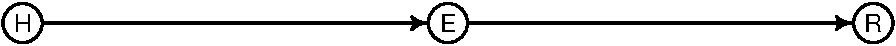
\includegraphics[width=0.5\linewidth,height=0.3\textheight]{ReplyToSteeleStefansson2_files/figure-latex/veracityDAG-1} \end{center}

The hypothesis node \(H\) bears on the whereabouts of the defendant.
Note the difference between \(E\) and \(R\). The evidence node bears on
what the witness saw. The reporting node bears on what the witness
reports to have seen. The chain of transmission from `seeing' to
`reporting' may fail for various reasons, such as lying or confusion.

Even if \textsc{Veracity} is a case of refinement, the old and new
probability functions agree with one another completely. The conditional
probabilities, \(\pr{E=e \vert H=h}\) should be the same as
\(\ppr{+}{E=e \vert H=h}\) for any values \(e\) and \(h\) of the
variables \(H\) and \(E\) that are shared before and after awareness
growth. In the Bayesian network, this falls out from its structure, as
the connection between \(H\) and \(E\) remains unchanged. Thus, Reverse
Bayesianism and Awareness Rigidity are perfectly fine in scenarios such
as \textsc{Veracity}.

A possible confusion should be eliminated at this point. We do not
intend to suggest that the assessment of the probability of the
hypothesis \textit{H=present} should undergo no change at all. If you
worry that the witness could have lied, shouldn't this affect your
belief in what they said about the defendant's whereabouts? Surely so.
But note that in \textsc{Veracity} an episode of awareness refinement
takes place together with a form of retraction. Initially, what is taken
to be known, after the learning episode, is that the witness
\textit{saw} the defendant around the crime scene. But after the growth
in awareness, you realize that your learning is in fact limited to what
the witness \textit{reported} to have seen. So the previous learning
episode is retracted and replaced by a more careful statement of what
you learned. This retraction will affect the probability you assign to
the hypothesis \textit{H=seen} conditional on your evidence, but this
does not conflict with Reverse Bayesianism or Awareness Rigidity, as you
re-conceptualized what your evidence actually is. In \textsc{Lighting},
instead, no retraction of the evidence takes place. The evidence that is
known remains the fact that the witness saw the defendant around the
crime scene, even though that experience could have been misleading due
to bad lighting conditions.

Where does this leave us? The following are now well-established: (a)
Reverse Bayesianism (or its close cousin Awareness Rigidity) handles
successfully at least some cases of awareness expansion; (b) it also
handles successfully at least some cases cases of refinement such as
\textsc{Veracity}; but (c) it does fail in cases of refinement like
\textsc{Lighting}. So, ultimately, Steele and Stefánsson's critique only
targets a subclass of refinement cases. The scope of this critique is
therefore somewhat limited. And yet, we do not think the prospects for
Reverse Bayesianism are good. In this respect, we tend to agree with
Steele and Stefánsson. But we conjecture that there is a deeper
difficulty for Reverse Bayesianism, besides possible counterexamples
that may be leveled against it. The deeper difficulty is that it seeks
to provide a formal, almost algorithmic solution to the problem of
awareness growth, and this formal aspiration is likely to lead us down
the wrong path.

To see why, consider again the distinction between the two cases of
refinement. Reverse Bayesianism is perfectly fine in scenarios like
\textsc{Veracity}, but fails in scenarios like \textsc{Lighting}. Why is
that so? In one scenario, what the witness saw could have occurred under
good or bad lighting conditions; in the other, what the witness saw
could have been reported truthfully or untruthfully. The two scenarios
are structurally different, and this difference can be appreciated by
looking at the Bayesian networks used to model them. In
\textsc{Veracity}, the new node is added downstream. Since the
conditional probabilities associated with the upstream nodes are
unaffected, Reverse Bayesianism is satisfied. By contrast, in
\textsc{Lighting}, the new node is added upstream. Since the conditional
probabilities that are associated with the downstream nodes will often
have to change, Reverse Bayesianism fails here.

This discussion suggests a conjecture: structural---possibly
causal---features about how we conceptualize a specific scenario seems
to be the guiding principles about how we update the probability
function through awareness growth, not a formal principle like Reverse
Bayesianism. We further elaborate on this conjecture in the final
section by drawing on some examples from Anna Mathani.

\hypertarget{mathanis-examples}{%
\section{Mathani's examples}\label{mathanis-examples}}

\label{sec:mathani}

Mahtani offered the following counterexamples:

\begin{quote}
\textsc{Tenant}: You are staying at Bob's flat which he shares with his landlord. You know
that Bob is a tenant, and that there is only one landlord, and that this landlord also
lives in the flat. In the morning you hear singing coming from the shower room, and
you try to work out from the sounds who the singer could be. At this point you have
two relevant propositions that you consider possible, that it's the landlord singing ($Landlord$), or that Bob is the singer ($Bob$) \dots  the possibility suddenly occurs to you that there might be
another tenant living in the same flat, and that perhaps that is the person singing in the
shower ($Other$).
\end{quote}

\begin{quote} 
\textsc{Tenant}: You know that I am holding a fair ten pence coin which I am about to toss. You
have a credence of 0.5 that it will land $Heads$, and a credence of 0.5 that it will
land $Tails$. You think that the tails side always shows an engraving of a lion. So you
also  have a credence of 0.5 that it will land with the lion engraving face-up ($Lion$). You  become aware
that  there are some ten pence coins that have an engraving of Stonehenge on the tails side, so you consider the proposition that the toss will end up with Stonehenge face-up ($Stonegenge$).



\end{quote}

\noindent The problem for Reverse Bayesianism with \textsc{Tenant}
appears when you consider the proposition is that the singer is a tenant
(\(Tenant\)). Suppose you originally took
\(\mathsf{P}(Landlord) = \mathsf{P}(Bob) = .5\). Since \(Bob\) and
\(Tenant\) originally are the same fact, \(\mathsf{P}(Tenant)\) = .5.
Since these are propositions that you were originally aware of, they
should remain in the same proportion after your awareness grows, that is
you should have \(\ppr{+}{Landlord} = \ppr{+}{Tenant} = k\). But also
\(Bob\) and \(Tenant\), being the same fact, had the same probability,
so you should also have \(\ppr{+}{Bob} = \ppr{+}{Tenant} = k\). But now,
\(Other\) entails \(Tenant\) and \(Bob\) and \(Other\) is disjoint, so
it follows that \(\ppr{+}{Other} = 0\), clearly an undesired
consequence.

The problem for Reverse Bayesianism with \textsc{Tails} is that you
initially gave \(Tails\) and \(Lion\) the same credence so you should
have \(\ppr{+}{Tails} = \ppr{+}{Lion} = k\). But since \(Lion\) and
\(Stonehenge\) are incompatible and the latter entails \(Tails\), you
should have \ppr{+}{Stonehenge} = 0\$, again an undesirable conclusion.

How do we approach these two cases using Bayesian networks? Let's start
with \textsc{Tenants}. We start with the following DAG:

\begin{center}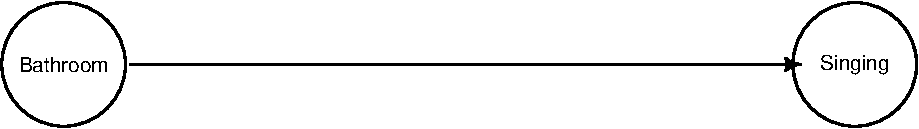
\includegraphics[width=0.5\linewidth,height=0.3\textheight]{ReplyToSteeleStefansson2_files/figure-latex/tenantsDAG-1} \end{center}

Initially, \(Bathroom\) has three possible states, representing who is
in the bathroom singing: \(landlord\), \(bob\), and \(noone\).
\(Singing\) is a binary node with two possible values: \(true\), and
\(false\). The original example is under-specified, so let's make some
probabilities and run with them. Suppose that both Bob and you have the
same probability of singing in the bathroom, say \(.2\). Also, quite
naturally, the probability of someone singing in an empty bathroom is 0.
Say also that the prior probability of you being in the bathroom is .1,
the same as the probability of the landlord being in the bathroom. Now
you learn \(Singing = true\) and update accordingly. The posterior
probabilities of \(bob\) and \(landlord\) now both equal .5, in line
with Mahtani's example. After your awarness grows, \(Bathroom\) now have
one more possible state, \(other\), which is also given prior
probability of \(.1\) (and the probability of \(noone\) drops from .8 to
.7). Now if you learn \(Singing = true\) and update, the posterior
probabilities of \(bob\), \(tenat\) and \(other\) all equal
\(\nicefrac{1}{3}\), which is exactly as desired.

There are two points here to observe. First, there is no magic in
modeling the problem with Bayesian networks. If somehow you know the
priors for the candidates are the same (which the example, we take,
already assumes), and assume the probabilities that Bob would sing or
that the landlord would sing in bathroom is not impacted by the new
possibility, the expected outcome falls out. Second, the assumptions
made and needed are non-trivial material assumptions that should not and
cannot fall out from purely formal considerations. As for priors, we can
easily imagine that landlord uses the bathroom in the mornings more
often, or tends to sing less. As for the impact of the new tenant, we
can also easily imagine circumstances in which Bob is less likely to
sing, say because now he is shy to sing in the presence of a new
flatmate.

The same two points can be made with respect to \textsc{Tails}. Now the
structure of the scenario is represented by the following DAG:

\begin{center}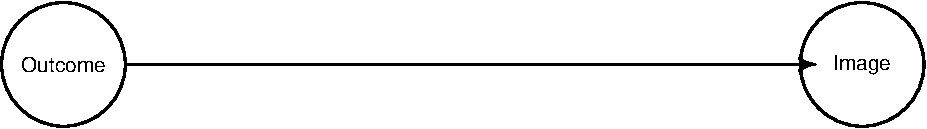
\includegraphics[width=0.5\linewidth,height=0.3\textheight]{ReplyToSteeleStefansson2_files/figure-latex/tailsDAG-1} \end{center}

\(Outcome\) has two states, \(tails\) and \(heads\). Initially, image
has two states too: \(none\) and \(lions\). We know that images have no
impact on the coin's fairness, so the priors for Outcome are \(.5\)
each, and this doesn't change once you learn something about other
images on the coin (again, a material assumption!). Initially, the
probability of \(none\) given \(heads\) is 1 and \(none\) given
\(tails\) is 0. Then you learn that not all images are those of a lion,
so you need some new probabilities (not given in the original example).
Say \(lion\) given \(tails\) has now the probability of \(.9\). What was
your original prior on \(lion\)? .5. What is it after the awareness
growth? .45. Again, no surprises in the construction, and again, how we
should build the network and which probabilities should shift is based
on our material knowledge that does not and should not fall out of
purely formal considerations.

\hypertarget{conclusion}{%
\section{Conclusion}\label{conclusion}}

We argued that Steele and Stefánsson's case against Reverse Bayesianism
is weaker than it might seem at first. The scenario
\textsc{Movies}---which is their key counterexample---is unconvincing
since it mixes learning and refinement. To avoid this, we constructed a
more clear-cut case of refinement, \textsc{Lighting}, in which both
Awareness Rigidity and Reverse Bayesianism fail unequivocally. At the
same time, we showed that there are cases of refinement like
\textsc{Veracity} in which Reverse Bayesianism and Awareness Rigidity
are perfectly fine in their place. ADD SOME BIT ABOUT HOW WE MODEL
MATHANI EXAMPLES

We conclude with a general moral. We think that the awareness of agents
grows while holding fixed certain material structural assumptions, based
on commonsense, semantic stipulations or causal dependency. To model
awareness growth, we need a formalism that can express these material
structural assumptions. This can done using Bayesian networks, and we
offered some illustrations of this strategy, for example, by distinguish
two forms of refinement on the basis of different structural
assumptions. These material assumptions also guide us in formulating the
adequate conservative constraints, and these will inevitably vary on a
case-by-case basis. Our approach stands in stark contrast with much of
the literature on awareness growth from a Bayesian perspective. This
literature is primarily concerned with a formal, almost algorithmic
solution to the problem. We suspect that seeking such formal solution is
doomed to fail. Insofar as Reverse Bayesianism is an expression of this
formalistic aspiration, we agree with Steele and Stefánsson that we are
better off looking elsewhere.

\end{document}
